% Analítica Predictiva y Prescriptiva · TIC-60286 · Semana 3
% Explorar con un agente
% Compilar: pdflatex week-03.tex (dos veces)
%
% Plan de los 90 minutos
%   0–5    Dónde vamos (láminas 2–3)
%   5–20   El paper: la fuga en las competencias de datos (láminas 4–8)
%  20–65   La aplicación: la demostración con el agente, el error sembrado,
%          la tabla cruzada a mano, los tres frenos, el sobre, las directivas,
%          privacidad, el giro (láminas 9–22)
%  65–70   Puente: el task 3 (lámina 23)
%  70–90   Cierre: el task 2, las matrices y la prueba de la fuente (lámina 24)
%
% Las cifras son las de datasets/aperturas/cifras_week03.txt (semilla de datos 18560).
% Las figuras de figures/ se copian de datasets/aperturas/figuras/ (las dibuja
% datasets/aperturas/_generar_estudio_aperturas.R).
% La demostración en vivo necesita: un agente con ejecución de código, la carpeta
% del proyecto (estudio_aperturas.csv, diccionario_estudio_aperturas.md,
% reglas_proyecto.md, el skill eda-con-agente) y el sobre de la semana 3 a la mano.
% El error sembrado es el paso 4 de la demostración (lámina 15): si el agente no
% propone solo el atraso de arriendo, se le pide "¿cuál es la variable que mejor
% separa a los que cerraron?" y lo hará.

\documentclass{beamer}
\input{../../_beamer/preambulo_app.tex}
\usetikzlibrary{calc}   % para centrar el nodo "Listo" bajo el bucle (lámina 9)
\semana{3}{Explorar con un agente}

\begin{document}

%%=================================================
%% Primer slide
\begin{frame}
\titlepage
\end{frame}

%% ====================================================== 0. DÓNDE VAMOS (0–5)
\begin{frame}{Dónde vamos}
\begin{columns}[T]
\begin{column}{0.5\textwidth}
\textbf{La semana pasada:} la vigilancia del entorno, la matriz de influencia y las dos incertidumbres críticas. Se discuten hoy, en el cierre.

\medskip
\textbf{Hoy, la pieza 3 del expediente:} los hallazgos de los datos. El estudio de aperturas (480 puntos de venta de conveniencia), explorado con un agente que escribe y corre el código, y una columna que hay que prohibir antes de modelar.
\end{column}
\begin{column}{0.5\textwidth}
\begin{block}{La sesión}
\begin{enumerate}
  \item El paper: la fuga que ganaba competencias de datos.
  \item Qué es un agente, en una lámina.
  \item La demostración en vivo, con un error sembrado.
  \item Los frenos, el sobre, las directivas, privacidad, el giro.
  \item Cierre: sus matrices y la prueba de la fuente.
\end{enumerate}
\end{block}
\end{column}
\end{columns}
\end{frame}

\begin{frame}{Antes de empezar}
\parada{encuesta}{¿Quién ha usado un agente que ejecuta código (Claude Code, Codex, Copilot en modo agente, el análisis de datos de un chat)? \quad (a) nunca \quad (b) lo he probado \quad (c) lo uso en el trabajo}
\medskip
Y una segunda, para quien marcó (b) o (c): ¿alguna vez le aceptaste una cifra sin ver el código que la produjo?
\end{frame}

\seccion{El paper: la fuga en las competencias de datos}
%% ====================================================== 1. EL PAPER (5–20)
\begin{frame}{El modelo que predecía el cáncer con el número del paciente}{Kaufman, Rosset y Perlich (2012), \emph{ACM Transactions on Knowledge Discovery from Data}}
\begin{columns}[T]
\begin{column}{0.5\textwidth}
\textbf{Qué investigaron.} Por qué los modelos que ganaban competencias de datos (KDD Cup, INFORMS) usaban, sin que nadie lo notara, información que \emph{no existiría} en el momento de predecir. Le pusieron nombre al fenómeno: \textbf{fuga} (\emph{leakage}), y propusieron cómo formularla, detectarla y evitarla.
\end{column}
\begin{column}{0.5\textwidth}
\textbf{El contexto.} En una competencia, miles de equipos reciben una base con la respuesta oculta y compiten por la mejor predicción. Si el ganador acierta porque encontró una pista que no estaría disponible en la vida real, el modelo no sirve para decidir nada, y nadie se entera hasta que se usa.
\end{column}
\end{columns}
\end{frame}

\begin{frame}{Qué datos y cómo}
\small
\begin{itemize}\itemsep5pt
  \item \textbf{KDD Cup 2008, cáncer de mama.} El objetivo era detectar imágenes con cáncer. El \textbf{número de identificación del paciente} resultó ser uno de los mejores predictores: los datos venían de varios centros con prevalencias distintas y los identificadores se habían asignado por bloques. El número no decía nada del paciente; decía de dónde venía la fila.
  \item \textbf{INFORMS 2008, neumonía.} Para armar la base le borraron a cada historia clínica el diagnóstico de neumonía. El hueco que dejó el borrado revelaba la respuesta.
  \item \textbf{El método.} Reunieron casos de varias competencias, formularon la condición de \textbf{legitimidad} de una variable (sin ``máquina del tiempo'': solo cuenta lo que existiría al predecir) y propusieron separar en el tiempo lo que se aprende de lo que se predice.
\end{itemize}
\end{frame}

\begin{frame}{Qué encontraron}
\begin{itemize}\itemsep6pt
  \item La fuga es \textbf{frecuente y silenciosa}: aparece por cómo se recogen y se arman los datos, no por mala fe, y ninguna métrica avisa.
  \item Una variable es legítima \textbf{solo si está disponible en el momento de la decisión}. No importa cuánto se correlacione con el resultado.
  \item La señal de alerta es un desempeño \textbf{demasiado bueno}: si un modelo acierta casi todo, lo primero no es celebrar; es buscar qué columna ya sabía la respuesta.
\end{itemize}
\medskip
\importa{Antes de leer un hallazgo, pregunta cómo se llenó cada columna y cuándo. La exploración (el EDA) es donde la fuga se atrapa: una variable que separa demasiado bien es sospechosa hasta que se demuestre lo contrario.}
\end{frame}

\begin{frame}{Por qué importa para quien decide}{Y una alternativa de negocios}
\begin{columns}[T]
\begin{column}{0.5\textwidth}
\begin{block}{El criterio del momento de la decisión}
Quien va a abrir un punto de venta no tiene los datos de los tres años siguientes. Todo lo que el modelo use tiene que existir \textbf{el día en que se firma el contrato}. Es el criterio que hoy atrapa a una columna del estudio de aperturas.
\end{block}
\end{column}
\begin{column}{0.5\textwidth}
\begin{exampleblock}{Lambrecht y Tucker (2019), \emph{Management Science}}
Un anuncio de empleos en ciencia y tecnología, diseñado para ser neutral, se les mostró a \textbf{menos mujeres} que hombres. No fue sesgo del algoritmo: mostrarle un anuncio a una mujer joven cuesta más, porque más anunciantes compiten por ella, y el sistema minimizaba costo. El dato decía ``discriminación''; el proceso que lo generó decía ``precios''.
\end{exampleblock}
\end{column}
\end{columns}
\smallskip
\small Las dos historias enseñan lo mismo: \textbf{antes de leer un hallazgo, pregunta cómo se llenaron los datos.}
\end{frame}

\begin{frame}{El puente}
\parada{el puente}{El estudio de aperturas trae 17 columnas y lo que le pasó a cada punto de venta a los tres años. ¿Y si una de esas columnas \textbf{ya sabe quién cerró}? ¿Cómo la reconocerías antes de que un agente la convierta en ``predictor estrella''?}
\medskip
\begin{itemize}
  \item Pista 1: el diccionario trae una columna que dice \emph{cuándo} se conoce cada variable.
  \item Pista 2: separa demasiado bien.
  \item Pista 3: para un local que todavía no abre, su valor es cero o no existe.
\end{itemize}
\end{frame}

\seccion{La aplicación: el EDA del estudio de aperturas con un agente}
%% ====================================================== 2. LA APLICACIÓN (20–65)
\begin{frame}{Qué es un agente, en una lámina}
\begin{columns}[T]
\begin{column}{0.52\textwidth}
\centering
\begin{tikzpicture}[
  caja/.style={draw=morado, fill=moradoclaro, rounded corners=4pt, text width=2.05cm, minimum height=1.05cm, align=center, font=\scriptsize},
  flecha/.style={-{Stealth[length=2.2mm]}, thick, morado},
  node distance=0.55cm and 0.45cm]
  \node[caja] (p) {\textbf{1. Planear}\\ lee la carpeta,\\ anuncia el plan};
  \node[caja, right=of p] (e) {\textbf{2. Ejecutar}\\ corre el script\\ en la terminal};
  \node[caja, below=of e] (o) {\textbf{3. Observar}\\ lee la salida real,\\ incluido el error};
  \node[caja, below=of p] (c) {\textbf{4. Corregir}\\ ajusta el código\\ con esa información};
  \draw[flecha] (p) -- (e);
  \draw[flecha] (e) -- (o);
  \draw[flecha] (o) -- (c);
  \draw[flecha] (c) -- (p);
  \node[draw=verdeosc, fill=verde!12, rounded corners=4pt, text width=4.4cm, align=center, font=\scriptsize, below=0.35cm of $(c.south)!0.5!(o.south)$] (l) {\textbf{Listo:} reporta la cifra con su fuente y lo que excluyó};
  \draw[flecha, verdeosc] (o.south) -- (l.north -| o.south);
\end{tikzpicture}
\end{column}
\begin{column}{0.48\textwidth}
\small
Un agente es un modelo de lenguaje con tres cosas más:
\begin{itemize}\itemsep3pt
  \item \textbf{contexto:} la carpeta del proyecto (la base, el diccionario, las reglas, la terminal);
  \item \textbf{manos:} ejecuta código de verdad;
  \item \textbf{el bucle:} prueba y corrige hasta que corre limpio.
\end{itemize}
\medskip
\importa{No es calculadora. Escribe el código, la máquina calcula, él lee y reporta. Si un número no salió de una ejecución, no existe.}
\end{column}
\end{columns}
\end{frame}

\begin{frame}{La demostración (1 de 4): el encargo y el prompt 0}
\small
\textbf{La carpeta del proyecto:} \texttt{estudio\_aperturas.csv} (480 puntos de venta, 17 columnas); \texttt{diccionario\_estudio\_aperturas.md}, con el \emph{momento} de cada columna (antes de abrir, después de abrir, target); \texttt{reglas\_proyecto.md}, las ocho reglas de la teoría; y el skill \texttt{eda-con-agente}, cargado.
\medskip
\begin{columns}[T]
\begin{column}{0.48\textwidth}
\begin{exampleblock}{Prompt 0}
``Lee \texttt{reglas\_proyecto.md} y el diccionario. No hagas cambios todavía. ¿Qué reglas del proyecto conoces?''
\end{exampleblock}
\end{column}
\begin{column}{0.52\textwidth}
\textbf{Qué debe pasar:} recita las reglas (una tarea por prompt, un script por resultado, ninguna cifra sin ejecución, pregunta antes de decidir) y dice qué columnas son de después de abrir.

\medskip
\textbf{Si no las recita,} no las leyó: se le vuelve a pedir antes de seguir.
\end{column}
\end{columns}
\end{frame}

\begin{frame}{La demostración (2 de 4): tu pregunta manda}
\begin{exampleblock}{Prompt 1}
\small ``La junta de Latitud evalúa abrir la primera tienda en Barranquilla. Mi pregunta: ¿qué perfil de local, entre los que se conocen \textbf{antes de abrir}, cierra menos y vende más? Con el diccionario, dime qué columnas sirven para esta pregunta y cuáles no. No escribas código todavía.''
\end{exampleblock}
\small
\textbf{Qué debe pasar:} nombra las doce columnas de antes de abrir, aparta las dos de después y los dos targets, y recuerda que Barranquilla no está en el estudio. Ojalá pregunte algo. No debe escribir código.
\smallskip
\parada{encuesta}{Antes de la primera cifra: ¿qué es una fila de \texttt{estudio\_aperturas.csv}? \quad (a) un punto de venta \quad (b) un punto de venta en un mes \quad (c) una ciudad \quad (d) un local candidato}
\medskip
Luego, el plan: ``Propón cuatro exploraciones, una línea cada una''. Yo recorto y reordeno. La regla de la sesión: \textbf{un prompt, una tarea, una ejecución, una mirada}.
\end{frame}

\begin{frame}{La demostración (3 de 4): el EDA, un prompt por paso}
\footnotesize
\begin{tabular}{@{}p{0.05\textwidth} p{0.34\textwidth} p{0.52\textwidth}@{}}
\toprule
 & El prompt pide & Lo que debe salir de la ejecución \\
\midrule
1 & ¿Qué es una fila? n, columnas, ids & 480 filas, 17 columnas, 480 ids distintos, sin faltantes \\
2 & El target: tasa de cierre y ventas típicas & 96 cierres de 480: \textbf{0.200}; mediana de ventas \textbf{95.0} \\
3 & La distribución de las ventas & media 100.7, máximo 259.0, el 10\,\% más alto pasa de 146.7: cola larga \\
4 & La tasa de cierre por zona, con conteo & residencial 0.289 (142), universitaria 0.234 (64), mixta 0.179 (151), oficinas 0.106 (123) \\
5 & La tasa de cierre por ciudad & de 0.180 (Cartagena) a 0.216 (Cali): plano \\
6 & Un cruce: tráfico bajo (menos de 120 personas por hora) & 0.528 (n = 53) frente a 0.159 en el resto \\
\bottomrule
\end{tabular}
\medskip

\parada{chat}{En cada paso, la misma pregunta: \textbf{¿esa cifra salió de código?} Si no vieron correr el script, escriban ``no''.}
\end{frame}

\begin{frame}{Las ventas: a la junta se le dice la mediana}
\begin{columns}[T]
\begin{column}{0.6\textwidth}
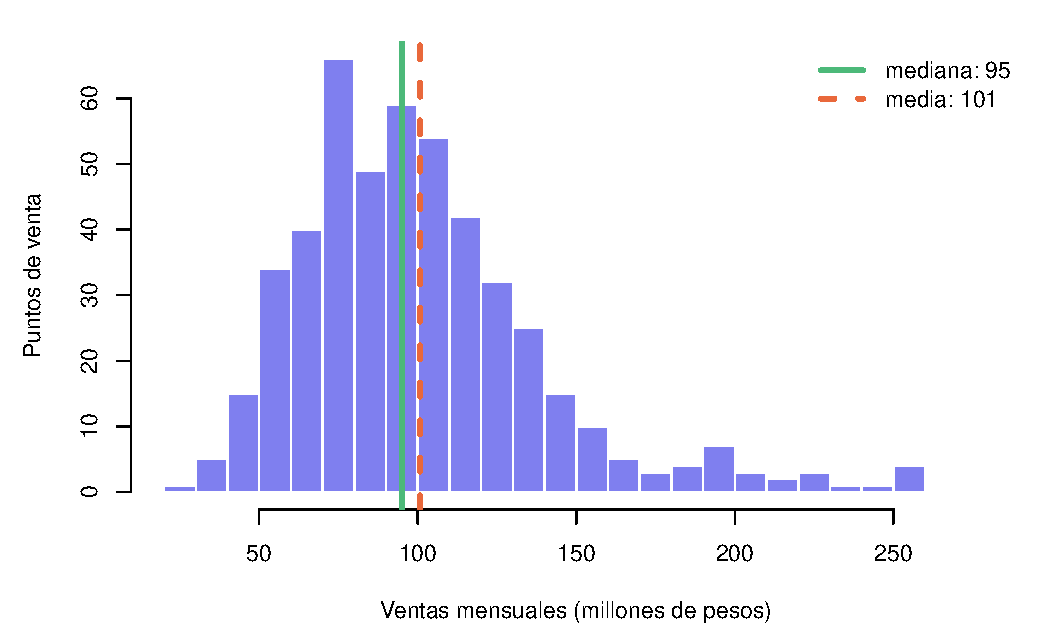
\includegraphics[width=\textwidth]{figures/eda_ventas_hist.pdf}
\end{column}
\begin{column}{0.4\textwidth}
\small
\begin{itemize}\itemsep4pt
  \item Mediana \textbf{95.0}, media \textbf{100.7}, máximo 259.0 millones al mes.
  \item 271 de los 480 puntos de venta venden menos que la media.
  \item ``Un punto de venta vende 100 millones'' hace que la junta espere más de lo que vende la mayoría.
\end{itemize}
\importa{La mediana, y mostrar la cola.}
\end{column}
\end{columns}
\end{frame}

\begin{frame}{Por zona separa; por ciudad, no}
\begin{columns}[T]
\begin{column}{0.5\textwidth}
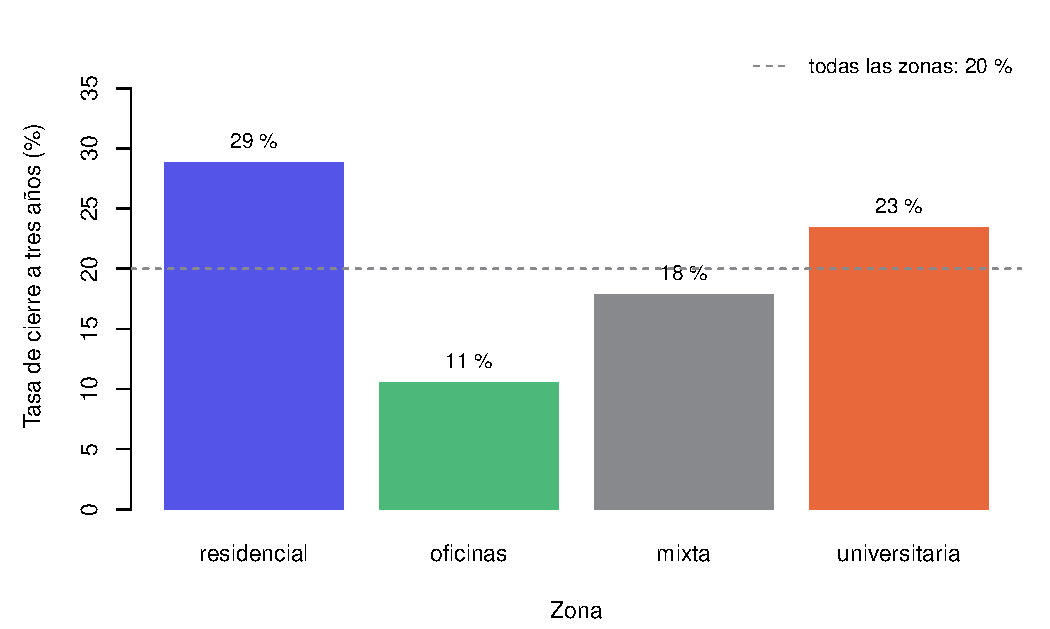
\includegraphics[width=\textwidth]{figures/eda_cierre_zona.pdf}

\small Residencial 0.289 frente a oficinas 0.106: dieciocho puntos que se conocen antes de firmar.
\end{column}
\begin{column}{0.5\textwidth}
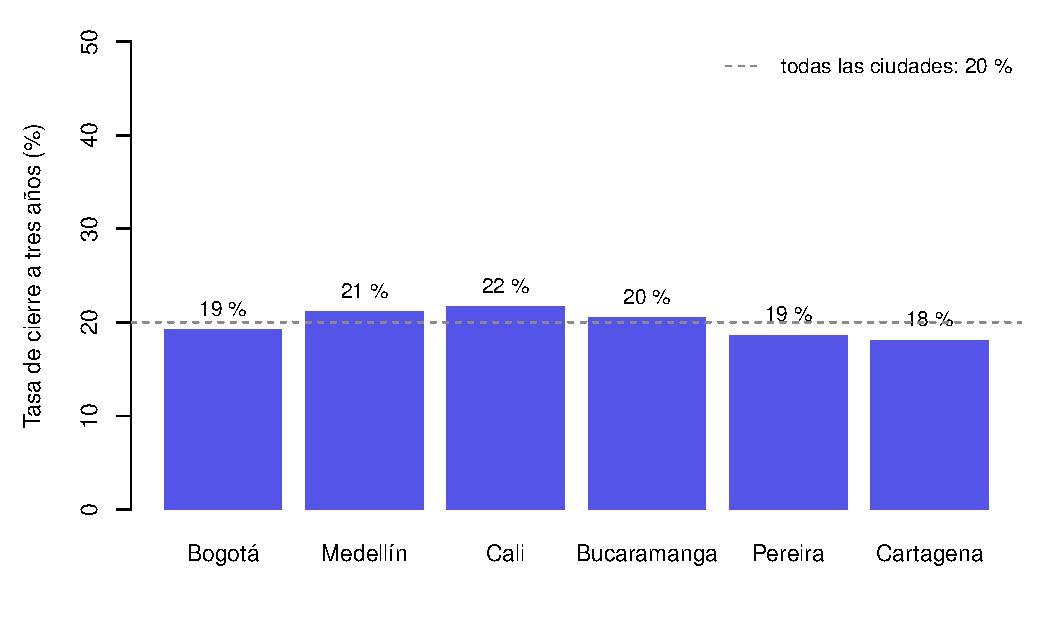
\includegraphics[width=\textwidth]{figures/eda_cierre_ciudad.pdf}

\small De 0.180 a 0.216, en la misma escala. \textbf{Un gráfico plano también es un hallazgo:} la ciudad no explica el cierre; el local sí.
\end{column}
\end{columns}
\end{frame}

\begin{frame}{La demostración (4 de 4): el hallazgo estrella}
\begin{exampleblock}{Prompt 7: ``¿Qué variable separa mejor a los que cerraron de los que siguen abiertos?''}
\small \textbf{El agente responde:} ``Hallazgo principal: de los puntos de venta con tres o más meses de atraso en el arriendo cerró el \textbf{89.7\,\%} (87 de 97); de los demás, el 2.3\,\% (9 de 383). Propongo \texttt{meses\_atraso\_arriendo} como predictor estrella del modelo de cierre.''
\end{exampleblock}
\medskip
\parada{el error sembrado}{Se detiene la demostración. La cifra es correcta: salió de código. ¿Esto sirve para un local que \textbf{todavía no abre}?}
\medskip
\small Pistas: ¿cuándo se acumula el atraso? ¿Cuántos meses de atraso tiene un local que no tiene contrato? ¿Qué dice el diccionario en la columna \emph{momento}?
\end{frame}

\begin{frame}{A mano: la tabla cruzada atraso por cierre}
\begin{columns}[T]
\begin{column}{0.52\textwidth}
\small
{\footnotesize\setlength{\tabcolsep}{4pt}%
\begin{tabular}{@{}l r r r@{}}
\toprule
Atraso de arriendo & Cerró & Abierto & Total \\
\midrule
3 meses o más & 87 & 10 & 97 \\
Menos de 3 meses & 9 & 374 & 383 \\
\midrule
Total & 96 & 384 & 480 \\
\bottomrule
\end{tabular}}
\medskip

Con atraso: $87 / 97 = 0.897$. \quad Sin atraso: $9 / 383 = 0.023$.

\medskip
Un local candidato de Barranquilla no tiene contrato: atraso \textbf{= 0}. Cae en la segunda fila. El ``predictor estrella'' les asigna a los tres locales el mismo 2.3\,\%.
\end{column}
\begin{column}{0.48\textwidth}
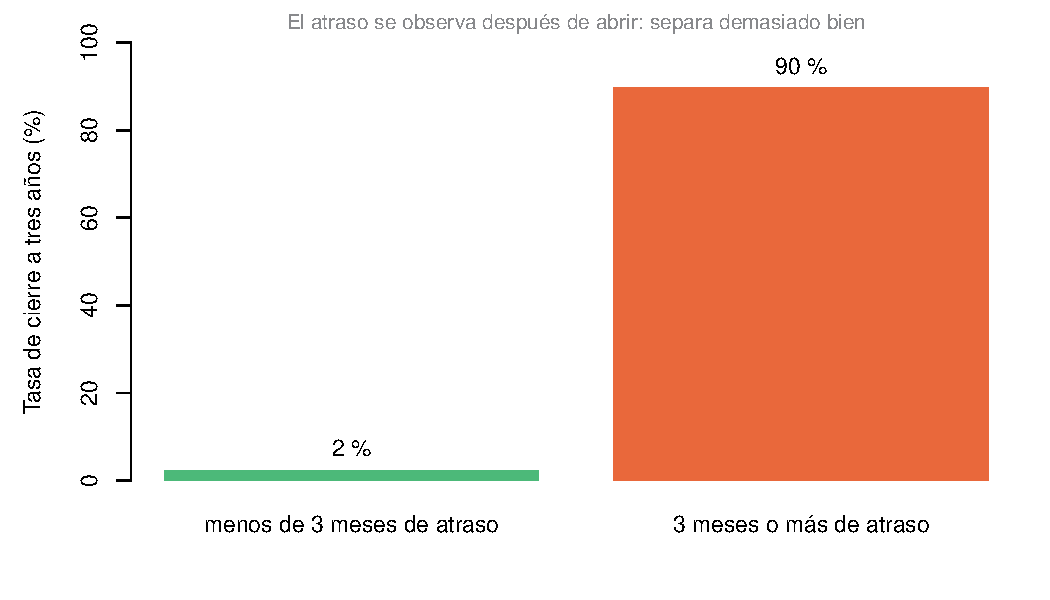
\includegraphics[width=\textwidth]{figures/eda_fuga.pdf}

\small La variable no predice el cierre: \textbf{lo acompaña}. Un punto de venta que va a cerrar deja de pagar el arriendo meses antes. Es la fuga de Kaufman, Rosset y Perlich, en una columna.
\end{column}
\end{columns}
\end{frame}

\begin{frame}{Los tres frenos, con la evidencia de hoy}
\footnotesize
\begin{tabular}{@{}p{0.29\textwidth} p{0.28\textwidth} p{0.31\textwidth}@{}}
\toprule
Lo que suele hacer el agente & Hoy pasó en\ldots & Lo que se le escribe \\
\midrule
\textbf{Hace de más:} pediste un paso y entregó el EDA completo, con un modelo de regalo & (marcar en vivo) & ``Hiciste más de lo que te pedí. Deja solo \emph{la tarea} y borra el resto.'' \\
\textbf{Inventa columnas:} usa \texttt{margen} o \texttt{rotacion}, que no están en el diccionario & (marcar en vivo) & ``No supongas los nombres. Lee el diccionario y usa los que existen.'' \\
\textbf{Afirma una cifra que no corrió:} ``la tasa de cierre es 19.8\,\%'' antes de ejecutar nada & (marcar en vivo) & ``¿De qué salida sale ese número? Muéstrame el código y córrelo.'' \\
\bottomrule
\end{tabular}
\medskip

\small Y un cuarto, el de hoy: \textbf{propone como predictor una columna de después de abrir.} ``Lista las columnas con momento `después de abrir' y exclúyelas antes de seguir.''
\end{frame}

\begin{frame}{La prueba del sobre: tres cifras del agente contra el sobre}
\small
\begin{tabular}{@{}p{0.27\textwidth} p{0.2\textwidth} p{0.12\textwidth} p{0.25\textwidth}@{}}
\toprule
Cifra & El agente dijo & El sobre & ¿Coincide o se explica? \\
\midrule
n, el grano de la tabla & \rule{0pt}{14pt} & 480 & \\
Tasa de cierre a tres años & \rule{0pt}{14pt} & 0.200 & \\
Mediana de ventas (millones al mes) & \rule{0pt}{14pt} & 95.0 & \\
\bottomrule
\end{tabular}
\medskip

\begin{block}{La regla del sobre}
La cifra del agente no vale hasta que coincide con la del sobre o se explica la diferencia: ``el agente dijo X, el sobre dice Y, y la diferencia venía de un filtro que aplicó, de filas que eliminó sin preguntar o de la media en lugar de la mediana''. Una cifra dicha antes de correr nada no se explica: es una alucinación numérica.
\end{block}
\end{frame}

\begin{frame}{Directivas que se pueden comprobar}
\parada{chat}{Escribe \textbf{una directiva verificable} para el agente del task 3: una regla que, al terminar, puedas comprobar en un minuto si se cumplió. Leemos cinco.}
\medskip
\small Tres vagas para reescribir, si hace falta inspiración:
\begin{itemize}\itemsep3pt
  \item ``Explora bien la base antes de modelar.''
  \item ``Sé riguroso con los valores atípicos.''
  \item ``Ten en cuenta que la decisión es abrir un local en Barranquilla.''
\end{itemize}
\medskip
Regla mental: dile al agente \textbf{qué} debe cumplirse, no \textbf{cómo} debe ser.
\end{frame}

\begin{frame}{Privacidad: analizar sin mirar}
\begin{columns}[T]
\begin{column}{0.5\textwidth}
\begin{block}{El chef sin nevera}
Le dan el menú, el inventario y las reglas de higiene, y le prohíben abrir la nevera. Diseña la receta completa porque conoce la \textbf{estructura} de los ingredientes, no los ingredientes.
\end{block}
\small En datos, la estructura es el \textbf{diccionario}: columnas, tipos, unidades, rangos y el momento en que se conoce cada una.
\end{column}
\begin{column}{0.5\textwidth}
\small
\textbf{Tres capas}
\begin{enumerate}\itemsep3pt
  \item Bloquear los archivos de datos: el agente escribe el código, lo corre quien tiene acceso.
  \item Diseñar el análisis sobre el diccionario: ningún registro individual viaja.
  \item Que la base calcule y devuelva solo agregados.
\end{enumerate}
\medskip
\importa{Los datos de tu empresa no se suben a un chat. En el memo individual trabajas con metadatos y diccionario, como el chef.}
\end{column}
\end{columns}
\end{frame}

\begin{frame}{El giro: la pregunta de la junta}
\parada{el giro}{La junta pregunta: ``¿Y la calificación de Google del local? En la base, los que cerraron tienen 3.77 estrellas y los que siguen abiertos 4.20; la correlación con el cierre es $-0.428$. ¿Por qué no la usan?''}
\medskip
\begin{itemize}\itemsep4pt
  \item Porque \textbf{nace después de abrir}: la ponen los clientes del punto de venta que ya opera. Para un local candidato no hay nada que consultar.
  \item El mismo criterio que para el atraso: \textbf{el momento de la decisión}, no la correlación.
  \item Lo que sí existe antes de abrir: la calificación de los \emph{competidores} del barrio, el tráfico, el arriendo, la zona. Eso entra al árbol de la semana 5.
\end{itemize}
\end{frame}

\begin{frame}{Lo que importa}
\importa{%
\begin{enumerate}\itemsep5pt
  \item \textbf{El agente no es calculadora.} Escribe el código, la máquina calcula, él reporta con su fuente. Una cifra sin ejecución no existe, y la del agente no vale hasta que coincide con el sobre o se explica.
  \item \textbf{Tú diriges.} Un prompt, una tarea, una ejecución, una mirada. Reglas cortas y verificables; tres frenos para cuando se desborda.
  \item \textbf{Una columna es legítima solo si existe en el momento de la decisión.} La que separa demasiado bien es sospechosa: pregunta cómo se llenó y cuándo.
\end{enumerate}}
\end{frame}

\seccion{El task y el cierre}
%% ====================================================== 3. PUENTE (65–70)
\begin{frame}{Task 3: tres hallazgos y una columna prohibida}
\small
\begin{columns}[T]
\begin{column}{0.55\textwidth}
\textbf{Qué se entrega} (una página, antes de la sesión 4; 5.0 puntos):
\begin{itemize}\itemsep2pt
  \item tres hallazgos con cifra y ``por qué importa'', y una figura cuyo título dice el hallazgo (2.0);
  \item las columnas que no se pueden usar, con el criterio del momento de la decisión (1.0);
  \item el acta: herramienta, prompts, qué verificaron contra las celdas de la teoría (1.0);
  \item qué hizo el agente de más o de menos (0.5); la declaración de IA (0.5).
\end{itemize}
Con un agente (el skill \texttt{eda-con-agente}) o con las celdas de la teoría: vale lo mismo.
\end{column}
\begin{column}{0.45\textwidth}
\begin{exampleblock}{En el cierre de la sesión 4: la cacería}
Se abre el sobre. Cada equipo compara sus cifras; dos equipos al azar muestran su figura; quién atrapó la fuga; cinco líneas de ``qué hizo el agente de más''.
\end{exampleblock}
\begin{alertblock}{Lo que no cuenta}
Una cifra que nadie vio correr. El atraso de arriendo como predictor. Una figura titulada ``Gráfico 1''.
\end{alertblock}
\end{column}
\end{columns}
\end{frame}

%% ====================================================== 4. CIERRE (70–90)
\begin{frame}{Cierre: el task 2, las matrices y la prueba de la fuente}
\begin{enumerate}\itemsep7pt
  \item \textbf{Dos equipos al azar, dos minutos cada uno} (6 minutos). El expositor también al azar. Muestran su matriz de influencia y su plano: qué quedó motriz, qué quedó crítico.
  \item \textbf{Por qué difieren} (5 minutos). Con las mismas variables, dos planos distintos: la diferencia es criterio, no error. ¿Qué celda explica la diferencia?
  \item \textbf{La prueba de la fuente, en vivo} (5 minutos). Una fila de la tabla de vigilancia de un equipo cualquiera: abrir el enlace, la fecha, quién publica, la frase exacta.
  \item \textbf{Las incertidumbres que se repiten} (4 minutos). ¿Qué dos incertidumbres críticas aparecen en más equipos? ¿Son irreducibles? Esas son las candidatas a ejes de la semana 7.
\end{enumerate}
\end{frame}

\begin{frame}{Referencias}
\small
\begin{itemize}\itemsep4pt
  \item Kaufman, S., Rosset, S., Perlich, C. y Stitelman, O. (2012). Leakage in data mining: formulation, detection, and avoidance. \emph{ACM Transactions on Knowledge Discovery from Data}, 6(4), artículo 15. (La versión de conferencia, KDD 2011, es de Kaufman, Rosset y Perlich.)
  \item Lambrecht, A. y Tucker, C. (2019). Algorithmic bias? An empirical study of apparent gender-based discrimination in the display of STEM career ads. \emph{Management Science}, 65(7), 2966--2981.
  \item Sosa Escudero, W. (2014). \emph{Qué es (y qué no es) la estadística}. Siglo XXI. El capítulo sobre correlación y causalidad.
  \item Latitud, gerencia de expansión (2026). \emph{Estudio de aperturas} (los datos del caso): \texttt{estudio\_aperturas.csv} y su diccionario, en la página de la semana 3.
\end{itemize}
\end{frame}

\end{document}
